\documentclass{mp}
\usepackage[linesnumbered]{algorithm2e}
\DontPrintSemicolon
\graphicspath{{15_prng}}
\subtitle{Generatory liczb pseudolosowych}

\SetKwProg{Fn}{Function}{}{end}
\SetKwInput{Assert}{assert}

\usepackage{alltt}

\usepackage{listings}
\lstdefinelanguage{C99}[]{C}{morekeywords={uint64\_t, uint32\_t, uint16\_t}}

\usepackage{tikzsymbols}

\newcommand{\xor}{\oplus}
\renewcommand{\vec}[1]{\mathbf{#1}}
\newcommand{\diag}[1]{\vec{D_{#1}}}

\usepackage{lstlinebgrd} % see http://www.ctan.org/pkg/lstaddons

%http://tex.stackexchange.com/questions/8851/how-can-i-highlight-some-lines-from-source-code
\makeatletter
%%%%%%%%%%%%%%%%%%%%%%%%%%%%%%%%%%%%%%%%%%%%%%%%%%%%%%%%%%%%%%%%%%%%%%%%%%%%%%
%
% \btIfInRange{number}{range list}{TRUE}{FALSE}
%
% Test in int number <number> is element of a (comma separated) list of ranges
% (such as: {1,3-5,7,10-12,14}) and processes <TRUE> or <FALSE> respectively

\newcount\bt@rangea
\newcount\bt@rangeb

\newcommand\btIfInRange[2]{%
    \global\let\bt@inrange\@secondoftwo%
    \edef\bt@rangelist{#2}%
    \foreach \range in \bt@rangelist {%
        \afterassignment\bt@getrangeb%
        \bt@rangea=0\range\relax%
        \pgfmathtruncatemacro\result{ ( #1 >= \bt@rangea) && (#1 <= \bt@rangeb) }%
        \ifnum\result=1\relax%
            \breakforeach%
            \global\let\bt@inrange\@firstoftwo%
        \fi%
    }%
    \bt@inrange%
}
\newcommand\bt@getrangeb{%
    \@ifnextchar\relax%
        {\bt@rangeb=\bt@rangea}%
        {\@getrangeb}%
}
\def\@getrangeb-#1\relax{%
    \ifx\relax#1\relax%
        \bt@rangeb=100000%   \maxdimen is too large for pgfmath
    \else%
        \bt@rangeb=#1\relax%
    \fi%
}

%%%%%%%%%%%%%%%%%%%%%%%%%%%%%%%%%%%%%%%%%%%%%%%%%%%%%%%%%%%%%%%%%%%%%%%%%%%%%%
%
% \btLstHL<overlay spec>{range list}
%
% TODO BUG: \btLstHL commands can not yet be accumulated if more than one overlay spec match.
% 
\newcommand<>{\btLstHL}[1]{%
  \only#2{\btIfInRange{\value{lstnumber}}{#1}{\color{color4!30}\def\lst@linebgrdcmd{\color@block}}{\def\lst@linebgrdcmd####1####2####3{}}}%
}%
\makeatother



\begin{document}
\frame{\titlepage}
\begin{frame}{9}
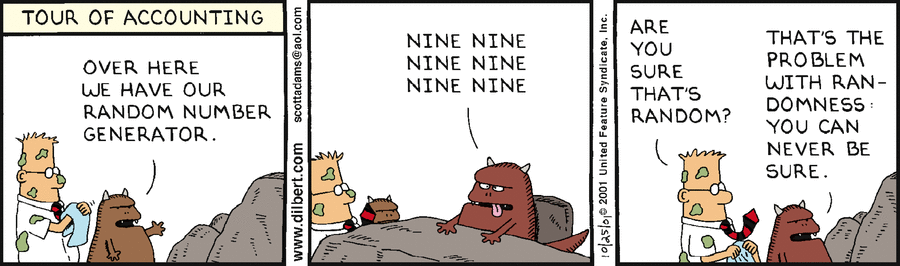
\includegraphics[width=\textwidth]{15_prng/dilbert.png}
\vfill
{\small \url{http://dilbert.com/strip/2001-10-25}}
\end{frame}
\begin{frame}{Ciąg liczb losowych}
\[ (X_1, X_2, \ldots) \]
\pause
\begin{enumerate}
\item $X_i$ mają identyczne rozkłady
\item $X_i$ są niezależne
\end{enumerate}
\end{frame}
\begin{frame}{Generowanie liczb o zadanym rozkładzie}
\begin{description}
\item[wejście] $X\sim\mathcal{U}(0,1)$
\item[wyjście] $Y$ z zadanego rozkładu
\end{description}
\pause
\[ Y=F^{-1}(X) \]
\pause
\[Y\sim Exp(0{,}5) \qquad x=0{,}1563 \]
\note<1>{\[F(y)=1-e^{-\lambda y} \qquad y=
\frac{\ln(1-F(y)}{-\lambda}=
\frac{\ln(1-0{,}1563}{-0{,5}}\approx 0{,}34\]}
\end{frame}
\begin{frame}{A jeżeli odwrotność $F$ nie jest znana?}
\begin{minipage}{.49\textwidth}
\begin{algorithm}[H]
\Repeat{$b-a\leq \delta$}
{
$y\leftarrow \frac{a+b}{2}$ \;
\lIf{$F(y)\leq X$}{$a\leftarrow y$}
\lElse{$b\leftarrow y$}
}
\Return{$y$}
\end{algorithm}
\end{minipage}
\begin{minipage}{.49\textwidth}
\pause
$Y\sim\mathcal{N}(0,1) \qquad x=0{,}1563$ \\
\pause
\begin{tabular}{rrrr}
	$a$	& $b$	& $y$ &	$F(y)$ \\
	\hline
$-10{,}000$	& $10{,}000$ &	$ 0{,}000$ & $0{,}500$ \\
\pause
$-10{,}000$	& \alert{$ 0{,}000$} &	$-5{,}000$ & $0{,}000$ \\
\alert{$ -5{,}000$}	& $ 0{,}000$ &	$-2{,}500$ & $0{,}006$ \\
\alert{$ -2{,}500$}	& $ 0{,}000$ &	$-1{,}250$ & $0{,}106$ \\
\alert{$ -1{,}250$}	& $ 0{,}000$ &	$-0{,}625$ & $0{,}266$ \\
$ -1{,}250$	& \alert{$-0{,}625$} &	$-0{,}938$ & $0{,}174$ \\
$ -1{,}250$	& \alert{$-0{,}938$} &	$-1{,}094$ & $0{,}137$ \\
\alert{$ -1{,}094$}	& $-0{,}938$ &	$-1{,}016$ & $0{,}155$ \\
\alert{$ -1{,}016$}	& $-0{,}938$ &	$-0{,}977$ & $0{,}164$ \\
$ -1{,}016$	& \alert{$-0{,}977$} &	$-0{,}996$ & $0{,}160$ \\
$ -1{,}016$	& \alert{$-0{,}996$} &	$-1{,}006$ & $0{,}157$ \\
$ -1{,}016$	& \alert{$-1{,}006$} &	$-1{,}011$ & $0{,}156$ \\
\alert{$ -1{,}011$}	& $-1{,}006$ &	$-1{,}008$ & $0{,}157$ \\
\end{tabular}
\end{minipage}
\end{frame}
\begin{frame}{A dla rozkładów dyskretnych?}
\begin{minipage}{.49\textwidth}
\begin{algorithm}[H]
$i\leftarrow 1$\;
$s\leftarrow p_1$ \;
\While{$s< X$}
{
$i \leftarrow i+1$\;
$s \leftarrow s+p_i$\;
}
\Return{$y_i$}
\end{algorithm}
\end{minipage}
\pause
\begin{minipage}{.49\textwidth}
$Y\sim \mathcal{B}(30,0{,}3) \qquad x=0{,}1563$ \\
\pause
\begin{tabular}{rrr}
$i=y$ &	$p_i$	& $s$ \\
$1$ & $0{,}000$ & $0{,}000$ \\
\pause
$2$ & $0{,}002$ & $0{,}002$ \\
$3$ & $0{,}007$ & $0{,}009$ \\
$4$ & $0{,}021$ & $0{,}030$ \\
$5$ & $0{,}046$ & $0{,}077$ \\
$6$ & $0{,}083$ & \alert{$0{,}160$} \\
\end{tabular}
\end{minipage}
\end{frame}

\begin{frame}[fragile]{Przypadek szczególny: skrócony rozkład równomierny}
\begin{description}
\item[wejście] $X\sim\mathcal{U}(0,n)$
\item[wyjście] $Y\sim\mathcal{U}(0,m)$
\end{description}
\pause
\begin{lstlisting}[language=Java,linebackgroundcolor={\btLstHL{3}}]
r = new Random(1);
for(int i=0;i<200000*11;i++)
    tab[i] = r.nextInt() % 11;
\end{lstlisting}
\pause
\begin{center}
\includegraphics[width=.6\textwidth]{15_prng/lcg_mod_11_hist.pdf}
\end{center}
\end{frame}
\begin{frame}[fragile]{Przypadek szczególny: skrócony rozkład równomierny}
\begin{lstlisting}[language=Java,linebackgroundcolor={\btLstHL{3}}]
r = new Random(1);
for(int i=0;i<200000*11;) {
    tab[i] = r.nextInt() & 0b1111;
    if(tab[i]<11) i++;
}
\end{lstlisting}
\pause
\vspace{-8mm}
\begin{center}
\includegraphics[width=.7\textwidth]{15_prng/lcg_mod_11_cut_hist.pdf}
\end{center}
\end{frame}
\begin{frame}{To samo z bliska}
\centering
\includegraphics[width=\textwidth]{15_prng/lcg_mod_11_comp.pdf}
\end{frame}
\begin{frame}{Analiza algorytmu}
\begin{description}
\item[wejście] $X_i\sim\mathcal{U}(0,2^n-1)\quad X_i$ niezależne
\item[wyjście] $(Y_1, Y_2, \ldots, Y_l)$\qquad $Y_j\sim\mathcal{U}(0,k-1)\quad 2^{n-1}<k\leq 2^n-1$
\end{description}
\pause
\alert{Ile potrzebujemy liczb na wejściu, żeby wygenerować $l$ liczb na wyjściu?}
\note<2>
{
\tiny
Żeby wygenerować jedną liczbę potrzebujemy $N$ liczb z wejścia, gdzie $N$ ma rozkład geometryczny (pobieramy $X$y do pierwszego sukcesu) z $p=\frac{k}{2^n}$.
Żeby wygenerować $l$ takich liczb, musimy zsumować $l$ zmiennych o takim rozkładzie: $W=N_1+N_2+\ldots+N_l$.
Te zmienne są niezależne, ponieważ $X$y są niezależne.
$EN_i=\frac{1}{p}=\frac{2^n}{k}$, $D^2N_i=\frac{1}{p^2}-\frac{1}{p}=\frac{2^n(2^n-k)}{k^2}$
Z niezależności $EN=l\frac{2^n}{k}$ i $D^2N=l\frac{2^n(2^n-k)}{k^2}$.
Nierówność Czebyszewa:
\[ P(N-EN\geq \varepsilon) \leq P(lstlisting\left|N-EN\right|\geq \varepsilon)\leq \frac{D^2N}{\varepsilon^2} \]
Niech $\varepsilon=l\varrho$ i $k=2^{n-1}$ (najgorszy możliwy przypadek):
\[ P(N-EN\geq \varepsilon) = P(N\geq l(\frac{2^n}{k}+\varrho)) = P(N\geq l(2+\varrho)) \leq \frac{l2^n2^{n-1}}{2^{2(n-1)}l^2\varrho^2}=\frac{2}{l\varrho^2}  \]
Niech $\varrho=8$ i wtedy $P(N\geq 10l)\leq \frac{1}{32l}$
}
\end{frame}
\begin{frame}{Ciąg liczb losowych}
\[ (X_1, X_2, \ldots) \]
\begin{enumerate}
\item \alert{$X_i\sim\mathcal{U}(0,n)$}  lub \alert{$X_i\sim\mathcal{U}(0,1)$}
\item $X_i$ są niezależne
\end{enumerate}
\end{frame}
\begin{frame}{Linear Congruential Generator (LCG)}
\begin{align*}
X_0 = & \text{seed} \\
X_{n+1} = & (aX_n+c) \mod m
\end{align*}
\end{frame}
\begin{frame}{Równomierność}
\centering
\only<1>{\includegraphics[width=.9\textwidth]{15_prng/lcg_1229_1_2048_hist.pdf}}
\only<2>{\includegraphics[width=.9\textwidth]{15_prng/lcg_65538_2_5040_hist.pdf}}
\only<3>
{
\begin{enumerate}
\item 247, 460, 93, 1658, 1971, 1624, 1145, 230, 47, 420, 85, 18, 1643, 1968, 2033, 2046, 1639, 1148, 1869
\item 362, 1478, 1406, 110, 1982, 398, 2126, 2990, 3422, 1118, 5006, 4430, 4142, 3998, \alert{1406, 110, 1982, 398, 2126}
\end{enumerate}
}
\end{frame}
\begin{frame}{Zasady doboru współczynników}
\begin{block}{Twierdzenie}
LCG ma okres $m$ wtedy i tylko wtedy gdy jednocześnie:
\begin{itemize}
\item $m$ i $c$ są względnie pierwsze,
\item $a-1$ jest podzielne przez wszystkie czynniki pierwsze $m$,
\item $a-1$ jest podzielne przez 4 jeżeli $m$ jest podzielne przez 4.
\end{itemize}
\end{block}
\pause
\begin{minipage}{.49\textwidth}
\includegraphics[width=\textwidth]{15_prng/lcg_1229_1_2048_hist.pdf}
\end{minipage}
\begin{minipage}{.49\textwidth}
\begin{tikzpicture}
    \node[anchor=south west,inner sep=0] (image) at (0,0) {\includegraphics[width=\textwidth]{15_prng/lcg_65538_2_5040_hist.pdf}};
    \begin{scope}[x={(image.south east)},y={(image.north west)}]
    	\draw[color4,very thick] (.05,.05) -- (.95,.95);
    	\draw[color4,very thick] (.05,.95) -- (.95,.05);
	\end{scope}
\end{tikzpicture}
\end{minipage}
\end{frame}

\begin{frame}{Zajrzyjmy do kodu}
\url{grepcode.com/file/repository.grepcode.com/java/root/jdk/openjdk/8u40-b25/java/util/Random.java\#Random.next\%28int\%29}
{
\small
\lstinputlisting[language=Java, firstline=88, lastline=90]{15_prng/Random.java}
\ldots
\lstinputlisting[language=Java, firstline=198, lastline=206]{15_prng/Random.java}
}
\end{frame}

\begin{frame}{Niezależność w LCG}
\begin{block}{Ciąg liczb losowych}
\[ (X_1, X_2, \ldots) \]
\begin{enumerate}
\item $X_i\sim\mathcal{U}(0,n)$  lub $X_i\sim\mathcal{U}(0,1)$
\item \alert{$X_i$ są niezależne}
\end{enumerate}
\end{block}
\[ P(X_{n+1}=7|X_n=7) = \alert{\ldots} \]
\pause
\[ P(X_{n+1}=7 \cup X_{n+2}=7 \cup \ldots \cup X_{n+m-1}=7|X_n=7) = \alert{\ldots} \]
\pause
\[ P(X_{n+m}=7|X_n=7) = \alert{\ldots} \]
\end{frame}


\begin{frame}{Multiply-with-carry}
\begin{align*}
(X_0, C_0) = & \text{seed} \\
\only<2->{\alert{\to}\,}X_{n+1} = & aX_n+C_n\mod b \\
C_{n+1} = & \left\lfloor\frac{aX_n+C_n}{b}\right\rfloor \\
\end{align*}
\begin{block}<3->{Uwaga}
seed \emph{nie} może być $(0, 0)$ ani $(a-1, b-1)$
\end{block}
\end{frame}

\begin{frame}{Dobór parametrów MWC}
\note<1>
{
$k$ jest rzędem $b$ w grupie $\mathbb{Z}_m$. $(C_n,X_n)$ ma pełen okres wtw $k=ab-2$.
Niestety, nie wynikają z tego żadne porządne własności $X_n$.
Przykładowo, dla $a=12$, $b=29$ rząd jest 173
}
\begin{block}{Twierdzenie (o rozkładzie)}
Niech $k\in\{2,3,\ldots, ab\}$ będzie najmniejszą liczbą taką, że 
\[b^k\mod (ab-1)=1\] 
Jeżeli $k=ab-2$, to MWC ma okres $k$ (maksymalny możliwy) i $aX_n+C_n\sim\mathcal{U}(1, ab-2)$.
\end{block}
\pause
\alert{Jaki rozkład ma zmienna $X_n$, jeżeli parametry zapewniają pełen okres?}
%\begin{block}{Wniosek o $X_n$}
%\centering
%\Sadey[5]
%\end{block}
\note<2>{
Skoro $aX_n+C_n\sim\mathcal{U}(1, ab-2)$, to $X_{n+1}=(aX_n+C_n)\mod b$ nie może mieć rozkładu jednostajnego, ponieważ zbiór możliwych wartości dla $aX_n+C_n$, tzn. $\{1,2,\ldots,ab-1\}$, ma $ab-2$ elementy, a więc liczbę niepodzielną bez reszty przez $b$.
W zbiorze brakuje elementu o reszcie $0$ (elementu $0$) i elementu o reszcie $b-1$, tzn. $ab-1$.
Inaczej: każda możliwa reszta występuje w zbiorze $a$ krotnie, natomiast $0$ i $b-1$ występują w nim $a-1$ krotnie.
Dla dużego $a$ z praktycznego punktu widzenia rozbieżność jest pomijalnie mała.

Empiryczna obserwacja na bazie parametrów $(6,10)$, $(6, 78)$ i $(10, 162)$: rozkład jest delikatnie nierównomierny, wartości od $1$ do $b-2$ pojawiają się z prawdopodobieństwem $\frac{a}{ab-2}$, natomiast $0$ i $b-1$ z prawdopodobieństwem $\frac{a-1}{ab-2}$.
}
\end{frame}

\begin{frame}[fragile]{Implementacja}
\begin{lstlisting}[language=C99]
//seed
uint16_t c=10;
uint16_t x=123;

uint16_t next()
{
        uint32_t t=a*x+c;
        c = t>>16;
        x = t&0xFFFF;
        return x;
}
\end{lstlisting}
\pause %
\begin{block}{Przykre twierdzenie}
Generator MWC dla którego $b=2^{2u}$ \emph{nie} może mieć pełnego okresu.
\end{block}
%TODO dlaczego?
\end{frame}

\begin{frame}{Przypomnienie wiadomości o macierzach}
%TODO
\end{frame}

\begin{frame}{XOR}
\centering
\begin{tabular}{cc|c}
$p$ & $q$ & $p\xor q$ \\
\hline
0 & 0 & \uncover<2->{0} \\
0 & 1 & \uncover<2->{1} \\
1 & 0 & \uncover<2->{1} \\
1 & 1 & \uncover<2->{0} \\
\end{tabular}

\vspace{1cm}
\begin{onlyenv}<3->
\begin{columns}[T]
\begin{column}{.49\textwidth}
\vspace{.5cm}
\begin{tabular}{c|c|cccc}
$x$ & 9 & 1 & 0 & 0 & 1 \\
$y$ & 5 & 0 & 1 & 0 & 1 \\
\hline
$x\xor y$ & \alt<5->{12}{\alert{\ldots}} 
&
\alt<-3>{\alert{\ldots}}{1 & 1 & 0 & 0}
\end{tabular}
\end{column}
\begin{column}{.49\textwidth}
\only<6->
{
\begin{align*}
\vec{x} = & [1, 0, 0, 1] \\
\vec{y} = & [0, 1, 0, 1] \\
\alert{\vec{x}+\vec{y}} = & [1, 1, 0, 0]
\end{align*}
}
\end{column}
\end{columns}
\end{onlyenv}
\end{frame}

\begin{frame}{SHL}
\centering
\begin{tabular}{l|c|cccc}
\texttt{y} & 9 & 1 & 0 & 0 & 1 \\
\texttt{y<<1} & \alt<3->{2}{\ldots} & \alt<2->{0 & 0 & 1 & \alert<2>{0}}{\alert{\ldots}} \\
%\only<4->{$y>>1$ & \alt<6->{4}{\ldots} & \alt<5->{\alert<5>{0} & 1 & 0 & 0}{\alert{\ldots}}} \\
\end{tabular}

\begin{onlyenv}<4->
\begin{align*}
\vec{y} = & [1, 0, 0, 1] = [y_3, y_2, y_1, y_0] \\
\vec{y}\vec{L} = & [0, 0, 1, 0] = [y_2, y_1, y_0, 0] \\
\end{align*}
\end{onlyenv}
\begin{onlyenv}<5->
\begin{align*}
\vec{L} = & 
\alt<6->
{
\begin{bmatrix} 
0 & 0 & 0 & 0 \\
1 & 0 & 0 & 0 \\
0 & 1 & 0 & 0 \\
0 & 0 & 1 & 0 \\
\end{bmatrix} \\
}
{
\begin{bmatrix} 
\alert{?} & \alert{?} & \alert{?} & \alert{?} \\
\alert{?} & \alert{?} & \alert{?} & \alert{?} \\
\alert{?} & \alert{?} & \alert{?} & \alert{?} \\
\alert{?} & \alert{?} & \alert{?} & \alert{?} \\
\end{bmatrix} \\
}
\begin{bmatrix} y_3 & y_2 & y_1 & y_0 \end{bmatrix} & \begin{bmatrix} y_2 & y_1 & y_0 & 0 \end{bmatrix} \\
\end{align*}
\end{onlyenv}
\end{frame}

\begin{frame}{SHR}
\centering
\begin{tabular}{l|c|cccc}
\texttt{y} & 9 & 1 & 0 & 0 & 1 \\
\texttt{y>>1} & \alt<3->{4}{\ldots} & \alt<2->{\alert<2>{0} & 1 & 0 & 0}{\alert{\ldots}} \\
\end{tabular}

\begin{onlyenv}<4->
\begin{align*}
\vec{y} = & [1, 0, 0, 1] = [y_3, y_2, y_1, y_0] \\
\vec{y}\vec{R} = & [0, 1, 0, 0] = [0, y_3, y_2, y_1] \\
\end{align*}
\end{onlyenv}
\begin{onlyenv}<5->
\begin{align*}
\vec{R} = & 
\alt<6->
{
\begin{bmatrix} 
0 & 1 & 0 & 0 \\
0 & 0 & 1 & 0 \\
0 & 0 & 0 & 1 \\
0 & 0 & 0 & 0 \\
\end{bmatrix} \\
}
{
\begin{bmatrix} 
\alert{?} & \alert{?} & \alert{?} & \alert{?} \\
\alert{?} & \alert{?} & \alert{?} & \alert{?} \\
\alert{?} & \alert{?} & \alert{?} & \alert{?} \\
\alert{?} & \alert{?} & \alert{?} & \alert{?} \\
\end{bmatrix} \\
}
\begin{bmatrix} y_3 & y_2 & y_1 & y_0 \end{bmatrix} & \begin{bmatrix} 0 & y_3 & y_2 & y_1 \end{bmatrix} \\
\end{align*}
\end{onlyenv}
\end{frame}

\begin{frame}{Wielokrotne przesunięcia}
$$
\vec{R} = \begin{bmatrix} 
0 & 1 & 0 & 0 \\
0 & 0 & 1 & 0 \\
0 & 0 & 0 & 1 \\
0 & 0 & 0 & 0 \\
\end{bmatrix} 
\qquad
\vec{L} = \begin{bmatrix} 
0 & 0 & 0 & 0 \\
1 & 0 & 0 & 0 \\
0 & 1 & 0 & 0 \\
0 & 0 & 1 & 0 \\
\end{bmatrix}
$$
\only<2->{$$\vec{R}=\vec{L}^T$$}
\only<3->
{
\texttt{y>>n = ((y>>1)>>1)>>\ldots>>1} $=\vec{y}\cdot \vec{R}\cdot \vec{R}\cdot\ldots\cdot \vec{R}=\vec{y}\vec{R}^n$ \\
\texttt{y<<n = ((y<<1)<<1)<<\ldots<<1} $=\vec{y}\cdot \vec{L}\cdot \vec{L}\cdot\ldots\cdot \vec{L}=\vec{y}\vec{L}^n$ \\
}
\end{frame}

\begin{frame}[fragile]{Xorshift}
\begin{lstlisting}[language=C]
y^=y<<17;
\end{lstlisting}
\pause
\begin{lstlisting}[language=C]
y=y^(y<<17);
\end{lstlisting}
\pause
\[ \vec{y}=\vec{y}+\vec{y}\cdot \vec{L}^{17}=\vec{y}(\vec{I}+\vec{L}^{17}) \]
\pause
\note<1>{$m$ to liczba bitów na jakiej operujemy}
\begin{block}{Generator Xorshift}
\begin{gather*}
\vec{T} = (\vec{I}+\vec{T_1}^{a_1})(\vec{I}+\vec{T_2}^{a_2})\cdot\ldots\cdot(\vec{I}+\vec{T_l}^{a_l}) \\
\vec{T_i}\in \{\vec{L}, \vec{R}\} \quad a_i\in \{1,\ldots,m-1\} \\
\end{gather*}
\pause
\begin{align*}
\vec{X_0} = & \text{\textbf{seed}} \in \{0,1\}^m \\
\vec{X_{n+1}} = & \vec{X_n}\vec{T}
\end{align*}
\end{block}
\end{frame}
\begin{frame}[fragile]{Implementacja}
\begin{lstlisting}[language=C99]
uint32_t xorshift(uint32_t seed)
{
 seed^=seed<<2;
 seed^=seed>>7;
 seed^=seed<<9;
 return seed;
}
\end{lstlisting}
\end{frame}
%TODO sprawdzic praktycznie, bez tego sie nie odwaze tego pokazac.
%TODO np wydaje mi sie, ze potegowanie musi byc nad cialem macierzy binarnych
%\begin{frame}{Długość okresu generatora Xorshift}
%\begin{block}{Twierdzenie (o okresie)}
%Żeby generator \emph{Xorshift} na $m$ bitach mógł osiągnąć wszystkie wartości potrzeba i wystarcza, żeby $T^{2^m}=T$ i jednocześnie $T^k\neq T$ dla dowolnego $k\in\{2,\ldots,
%\end{block}
%\end{frame}
\begin{frame}{32-bitowy oraz 64-bitowy Xorshift}
\begin{block}{Twierdzenie (o długości)}
32-bitowy Xorshift ($m=32$) oraz 64-bitowy Xorshift ($m=64$) o pełnym okresie wymaga przynajmniej trzech przesunięć ($l\geq 3$) 
\end{block}
\pause
\begin{block}{Twierdzenie (o kierunkach)}
Jeżeli przesunięcia \texttt{<<a, >>b, <<c} zapewniają pełen okres, to dokonanie jednej lub kilku poniższych operacji nie zmieni długości okresu:
\begin{itemize}
\item odwrócenie kierunku wszystkich przesunieć
\item zamiana $a$ i $c$ miejscami
\item zamiana dwóch ostatnich przesunięć miejscami: \texttt{<<a, <<c, >>b}
\end{itemize}
\end{block}
\pause
\begin{block}{Twierdzenie (o współczynnikach)}
Istnieje dokładnie 81 trójek $(a,b,c)$ zapewniających pełen okres dla $m=32$ i $275$ trójek dla $m=64$.
\end{block}
\vfill
{\footnotesize G. Marsaglia \emph{Xorshift RNGs} w: \emph{Journal of Statistical Software} 8(14)}
\end{frame}
\begin{frame}{Trójki $(a,b,c)$ dla $m=32$}
\scriptsize
\begin{alltt}
| 1, 3,10| 1, 5,16| 1, 5,19| 1, 9,29| 1,11, 6| 1,11,16| 1,19, 3| 1,21,20| 1,27,27| \\
| 2, 5,15| 2, 5,21| 2, 7, 7| 2, 7, 9| 2, 7,25| 2, 9,15| 2,15,17| 2,15,25| 2,21, 9| \\
| 3, 1,14| 3, 3,26| 3, 3,28| 3, 3,29| 3, 5,20| 3, 5,22| 3, 5,25| 3, 7,29| 3,13, 7| \\
| 3,23,25| 3,25,24| 3,27,11| 4, 3,17| 4, 3,27| 4, 5,15| 5, 3,21| 5, 7,22| 5, 9,7 | \\
| 5, 9,28| 5, 9,31| 5,13, 6| 5,15,17| 5,17,13| 5,21,12| 5,27, 8| 5,27,21| 5,27,25| \\
| 5,27,28| 6, 1,11| 6, 3,17| 6,17, 9| 6,21, 7| 6,21,13| 7, 1, 9| 7, 1,18| 7, 1,25| \\
| 7,13,25| 7,17,21| 7,25,12| 7,25,20| 8, 7,23| 8,9,23 | 9, 5,1 | 9, 5,25| 9,11,19| \\
| 9,21,16|10, 9,21|10, 9,25|11, 7,12|11, 7,16|11,17,13|11,21,13|12, 9,23|13, 3,17| \\
|13, 3,27|13, 5,19|13,17,15|14, 1,15|14,13,15|15, 1,29|17,15,20|17,15,23|17,15,26| \\
\end{alltt}
\vfill
{\footnotesize G. Marsaglia \emph{Xorshift RNGs} w: \emph{Journal of Statistical Software} 8(14)}
\end{frame}
\begin{frame}{KISS: Keep it simple, stupid!}
\begin{align*}
X_{n+1} = & \left(69069 X_n + 12345\right) \mod 2^{32} \\
Y_{n+1} = & Y_n(I+L^{13})(I+R^{17})(I+L^5) \\
C_{n+1} = & \left\lfloor \frac{698769069Z_n+C_n}{2^{32}}\right\rfloor \\
Z_{n+1} = & \left(698769069Z_n+C_n\right) \mod 2^{32} \\
 & \alert{\left(X_{n+1}+Y_{n+1}+Z_{n+1}\right) \mod 2^{32}}
\end{align*}
\pause
\begin{block}{Hipoteza (G. Marsaglia)}
Okres generatora KISS jest dłuższy niż $2^{124}$
\end{block}
\note<2>
{
Wydaje mi się, że rozumowanie jest następujące: jeżeli generatory są niezależne, to możemy pomnożyć ich okresy. LCG i Xorshift mają po $2^{32}$, MWC ma (w wariancie optymistycznym, nie sprawdzałem czy tak jest w rzeczywistości) $698769069\cdot 2^{32}\cdot\frac{1}{2}-2\approx 2^{60}$, zatem cały generator ma okres $2^{32}\cdot 2^{32}\cdot 2^{60}=2^{124}$. $\frac{1}{2}$ bierze się z problemów z $b=2^{32}$.
}
\pause
\begin{block}{Twierdzenie}
Generator KISS ma rozkład równomierny.
\end{block}
\note<3>
{
\scriptsize
Dowód mojego autorstwa.
Rozpatrzmy dwie niezależne zmienne losowe $X, Y$ takie, że $X,Y \sim \mathcal{U}(0,2^{32}-1)$.
Niech $W=X+Y$, rozpatrujemy dwa przypadki:
\begin{enumerate}
\item $0\leq k< 2^{32}$
\[ P(W=k)=\sum_{x=0}^k P(X=x)P(Y=k-x) = \sum_{x=0}^k \frac{1}{2^{64}} = \frac{k+1}{2^{64}} \]
\item $2^{32}\leq k<2^64$, niech $k=2^{32}+l$ i wtedy $0\leq l<2^{32}$.
Chcemy sumować w taki sposób, żeby $0\leq x<2^{32}$ i $0\leq k-x<2^{32}$, rozwiązując nierówności otrzymujemy $x\in\{l+1,\ldots,2^{32}-1\}$
\[ 
\begin{split}
P(W=k)=\sum_{x=l+1}^{2^{32}-1} P(X=x)P(Y=k-x) = \frac{2^{32}-1-(l+1)+1}{2^64}= \\
\frac{1}{2^{32}}-\frac{(l+1)}{2^{64}}=\frac{1}{2^{32}}-P(W=l) 
\end{split}
\]
\end{enumerate}
Następnie rozpatrzmy $U=(X+Y)\mod 2^{32}$.
\[ P(U=k)=P(W=k)+P(W=k+2^{32})=P(W=k)+\frac{1}{2^{32}}-P(W=k)=\frac{1}{2^{32}} \]
W takim razie $U\sim\mathcal{U}(0,2^{32}-1)$.
Podstawiając $U$ jako $X$ otrzymujemy wnik dla sumy trzech zmiennych, czyli to, co dzieje się w KISS.
}
\end{frame}
\begin{frame}[fragile]{Implementacja KISS}
\small
\begin{lstlisting}[language=C99]
//seed
uint32_t x=123456789, y=362436000;
uint32_t z=521288629, c=7654321;

uint32_t KISS()
{
        x=69069*x+13245;

        y^=y<<13;
        y^=y>>17;
        y^=y<<5;

        uint64_t t=698769069;
        t=t*z+c;
        c=t>>32;

        return x+y+z;
}
\end{lstlisting}
\end{frame}
\begin{frame}{Mersenne twister}
\begin{block}{Oznaczenia}
\[ \vec{I}_r =  \overbrace{\begin{bmatrix} 
1 & 0 & \ldots & 0 \\
0 & 1 & \ldots & 0 \\
\hdotsfor{4} \\
0 & 0 & \ldots & 1 \\
\end{bmatrix}}^{r} 
\qquad
\diag{b} = \begin{bmatrix}
b_k & 0 & \ldots & 0 \\
0 & b_{k-1} & \ldots & 0 \\
\hdotsfor{4} \\
0 & 0 & \ldots & b_0
\end{bmatrix}
\]
\end{block}
\pause
\begin{block}{Postać ogólna}
\begin{align*}
\vec{X_{k+n}} = & \left(\vec{X_{k+m}} + \vec{X_{k+1}}\begin{bmatrix} 0 & 0 \\ 0 & \vec{I}_r \end{bmatrix}\vec{A} + \vec{X_k}\begin{bmatrix} \vec{I}_{w-r} & 0 \\ 0 & 0 \end{bmatrix}\vec{A}\right)\vec{T} \\
\vec{T} = & \vec{R}^u(\vec{L}^s\diag{b})(\vec{L}^t\diag{c})\vec{R}^l
\end{align*}
$\vec{A}, \vec{b}, \vec{c}, u, s, t, l, r, m$ to zdefiniowane stałe, $w$ to liczba bitów
\end{block}
\pause
\begin{tikzpicture}[overlay]
\draw[red,very thick] (current page.south west) -- (current page.north east);
\draw[red,very thick] (current page.north west) -- (current page.south east);
\end{tikzpicture}
\end{frame}
\begin{frame}{MT19937}
\begin{itemize}
\item Wyjątkowo długi okres $2^{19937}-1$ dla 32 bitowej wersji
\pause
\item Bardzo popularny, domyślny dla Pythona i PHP
\pause
\item Podobny do Xorshift
\pause
\item Odwracalny
\pause
\item Wyjściem jest cały stan
\pause
\item Używa jednocześnie 624 liczb
\pause
\item Implementacje często generują seed z jednej liczby
\end{itemize}
\end{frame}
\begin{frame}{Zajrzyjmy do kodu!}
\begin{itemize}
\item \url{https://en.wikipedia.org/w/index.php?title=Mersenne\_Twister&oldid=708041651\#Python\_implementation}
\item \url{https://hg.python.org/cpython/file/tip/Modules/_randommodule.c}, funkcja \texttt{genrand\_int32}
\end{itemize}
\end{frame}
\begin{frame}{Fortuna}
\begin{block}{Stan}
\begin{description}
\item[$C$] 128 bitowy licznik, monotoniczny
\item[$K$] 256 bitowy klucz, ciąg pseudolosowy
\end{description}
\end{block}
\begin{algorithm}[H]
\pause
\SetKwFunction{FortunaGenerate}{Generate}
\Fn{\FortunaGenerate{$n$}}
{
\Assert{$0\leq n\leq 2^{20}$}
$result \leftarrow []$ \;
\For{$k\leftarrow 1$ \KwTo $\lceil\frac{n}{16}\rceil$}
{
$result\leftarrow result\ ||\ \text{AES}(K, C)$ \;
$C\leftarrow C+1$ \;
}
$K\leftarrow \text{AES}(K, C)\ ||\ \text{AES}(K, C+1)$ \;
$C\leftarrow C+2$ \;
\Return{$result$} \;
}
\end{algorithm}
\note{Potrzebujemy regularnie wymieniać klucz, inaczej pojawią się statystycznie rozpoznawalne różnice, bo AES nie powtórzy bloku. Stąd ograniczenie do $2^{20}$.}
\end{frame}
\begin{frame}{Reseedowanie Fortuny}
\begin{block}{Dane}
\begin{description}
\item[$RC$] 32-bitowy licznik, początkowo $0$
\item[$P_0, \ldots, P_{31}$] pule entropii
\end{description}
\end{block}
\begin{algorithm}[H]
\SetKwFunction{FortunaReseed}{Reseed}
\Fn{\FortunaReseed{}}
{
$RC \leftarrow RC + 1$ \;
$s \leftarrow []$ \;
\For{$i\leftarrow 0$ \KwTo $31$}
{
\If{$2^i$ dzieli $RC$}
{
$s \leftarrow s\ ||\ \text{SHA}_{256}(P_i)$ \;
$P_i\leftarrow \emptyset$ \;
}
}
$K \leftarrow \text{SHA}_{256}(K\ ||\ s)$ \;
}
\end{algorithm}
\end{frame}
\begin{frame}{Fortuna z automatycznym reseedowaniem}
\begin{algorithm}[H]
\SetKwFunction{FortunaFullRandom}{FullRandom}
\Fn{\FortunaFullRandom{$n$}}
{
\If{w $P_0$ spodziewamy się dostatecznie dużo entropii i od ostatniego reseedowania upłynęło co najmniej 100 ms}
{
\FortunaReseed{} \;
$C\leftarrow C+1$ \;
}
\lIf{$C>0$}{\Return{\FortunaGenerate{$n$}}}
\lElse{\Return{błąd}}
}
\end{algorithm}
\note<1>{$100 ms\cdot 2^{32}\approx 13 lat$, więc tak łatwo nie wyczerpiemy zapasów}
\end{frame}
\begin{frame}{Źródła entropii}
\begin{itemize}
\item<+-> czas pomiędzy naciśnięciami klawiszy na klawiaturze, ruchami myszy
\item<+-> czas pomiędzy przybyciem pakietów sieciowych
\item<+-> czas pomiędzy przerwaniami sprzętowymi
\item<+-> precyzyjnie mierzony czas wykonania krótkiego, deterministycznego kodu (demon \emph{haveged})
\item<+-> generatory sprzętowe
\begin{itemize}
\item<+-> szumy termiczne
\item<+-> szum radiowy
\item<+-> rozpad promieniotwórczy
\item<+-> instrukcja \texttt{\textsc{rdseed}} (Intel)
\end{itemize}
\item<+-> Lotto
\begin{itemize}
\item<+-> w wielu krajach
\end{itemize}
\end{itemize}
\begin{block}<+->{Ciekawostka}
\texttt{\textsc{rdrand}} = algorytm zbliżony do Fortuny
\end{block}
\note<1>{\url{https://software.intel.com/en-us/articles/intel-digital-random-number-generator-drng-software-implementation-guide}}
\end{frame}
\begin{frame}{Dobre praktyki}
\begin{itemize}
\item Stosuj dobre generatory
\pause
\item W zastosowaniach mission-critical, stosuj generatory kryptograficznie bezpieczne
\pause
\item Rozgrzewaj generator
\pause
\item Wykorzystuj tylko mały fragment okresu generatora
\pause
\item Zapewnij dostatecznie dużą przestrzeń seedów
\only<5>
{
\begin{block}{Rzeczywisty problem z Florydy}
Ile jest możliwych wyborów 80 ławników z listy 200 kandydatów?
Czy ta liczba mieści się w 32-bitach? A 64-bitach?
\end{block}
}
\note<1>{\texttt{log2(nchoosek(200,80))=190}}
\pause
\item Dbaj o dobry wybór seeda
\only<6>
{
\begin{block}{Symulacja na klastrze}
Zlecamy 100 symulacji opartych na RNG do wykonania na klastrze, identyczne zadania.
Co się stanie jeżeli użyjemy \texttt{time()} jako seed?
\end{block}
}
\pause
\item W razie wątpliwości zajrzyj do E. Barker, J. Kelsey \emph{Recommendation for Random Number Generation Using Deterministic Random Bit Generators} (\emph{NIST Special Publication 800-90A})
\end{itemize}
\end{frame}
\begin{frame}{Bibliografia}
\begin{enumerate}
\item ,,The Art of Computer Programming'' (Vol. 2) D. Knuth, rozdział III
\item ,,Non-Uniform Random Variate Generation'' L. Devroye \url{http://www.nrbook.com/devroye/}
\item N. Ferguson, B. Schneier, T. Kohno \emph{Cryptography engineering} John Wiley \& Sons, 2010
\end{enumerate}
\end{frame}
\end{document}
